\documentclass[a4paper, 12pt]{article}

% packages
\usepackage{amssymb}
\usepackage[fleqn]{mathtools}
\usepackage{tikz}
\usepackage{enumerate}
\usepackage{bussproofs}
\usepackage{xcolor}
\usepackage[margin=1.3cm]{geometry}
\usepackage{logicproof}
\usepackage{diagbox}
\usepackage{listings}
\usepackage{graphicx}
\usepackage{lstautogobble}
\usepackage{hyperref}
\usepackage{multirow}
\usepackage{tipa}
\usepackage{pgfplots}

% tikz libraries
\usetikzlibrary{
    decorations.pathreplacing,
    arrows,
    shapes.gates.logic.US,
    circuits.logic.US,
    calc,
    automata,
    positioning,
    intersections
}

\pgfplotsset{compat=1.16}

\pgfmathdeclarefunction{gauss}{2}{%
  \pgfmathparse{1/(#2*sqrt(2*pi))*exp(-((x-#1)^2)/(2*#2^2))}%
}

\allowdisplaybreaks % allow environments to break
\setlength\parindent{0pt} % no indent

% shorthand for verbatim
% this clashes with logicproof, so maybe fix this at some point?
\catcode`~=\active
\def~#1~{\texttt{#1}}

% code listing
\lstdefinestyle{main}{
    numberstyle=\tiny,
    breaklines=true,
    showspaces=false,
    showstringspaces=false,
    tabsize=2,
    numbers=left,
    basicstyle=\ttfamily,
    columns=fixed,
    fontadjust=true,
    basewidth=0.5em,
    autogobble,
    xleftmargin=3.0ex,
    mathescape=true
}
\newcommand{\dollar}{\mbox{\textdollar}} %
\lstset{style=main}

% augmented matrix
\makeatletter
\renewcommand*\env@matrix[1][*\c@MaxMatrixCols c]{%
\hskip -\arraycolsep
\let\@ifnextchar\new@ifnextchar
\array{#1}}
\makeatother

% ceiling / floor
\DeclarePairedDelimiter{\ceil}{\lceil}{\rceil}
\DeclarePairedDelimiter{\floor}{\lfloor}{\rfloor}

% custom commands
\newcommand{\indefint}[2]{\int #1 \, \mathrm{d}#2}
\newcommand{\defint}[4]{\int_{#1}^{#2} #3 \, \mathrm{d}#4}
\newcommand{\pdif}[2]{\frac{\partial #1}{\partial #2}}
\newcommand{\dif}[2]{\frac{\mathrm{d}#1}{\mathrm{d}#2}}
\newcommand{\limit}[2]{\raisebox{0.5ex}{\scalebox{0.8}{$\displaystyle{\lim_{#1 \to #2}}$}}}
\newcommand{\limitsup}[2]{\raisebox{0.5ex}{\scalebox{0.8}{$\displaystyle{\limsup_{#1 \to #2}}$}}}
\newcommand{\summation}[2]{\sum\limits_{#1}^{#2}}
\newcommand{\product}[2]{\prod\limits_{#1}^{#2}}
\newcommand{\intbracket}[3]{\left[#3\right]_{#1}^{#2}}
\newcommand{\laplace}{\mathcal{L}}
\newcommand{\fourier}{\mathcal{F}}
\newcommand{\mat}[1]{\boldsymbol{#1}}
\renewcommand{\vec}[1]{\boldsymbol{#1}}
\newcommand{\rowt}[1]{\begin{bmatrix}
    #1
\end{bmatrix}^\top}
\DeclareMathOperator*{\argmax}{argmax}
\DeclareMathOperator*{\argmin}{argmin}

\newcommand{\lto}[0]{\leadsto\ }

\newcommand{\ulsmash}[1]{\underline{\smash{#1}}}

\newcommand{\powerset}[0]{\wp}
\renewcommand{\emptyset}[0]{\varnothing}

\makeatletter
\newsavebox{\@brx}
\newcommand{\llangle}[1][]{\savebox{\@brx}{\(\m@th{#1\langle}\)}%
  \mathopen{\copy\@brx\kern-0.5\wd\@brx\usebox{\@brx}}}
\newcommand{\rrangle}[1][]{\savebox{\@brx}{\(\m@th{#1\rangle}\)}%
  \mathclose{\copy\@brx\kern-0.5\wd\@brx\usebox{\@brx}}}
\makeatother
\newcommand{\lla}{\llangle}
\newcommand{\rra}{\rrangle}
\newcommand{\la}{\langle}
\newcommand{\ra}{\rangle}
\newcommand{\crnr}[1]{\text{\textopencorner} #1 \text{\textcorner}}
\newcommand{\bnfsep}[0]{\ |\ }
\newcommand{\concsep}[0]{\ ||\ }

\newcommand{\axiom}[1]{\AxiomC{#1}}
\newcommand{\unary}[1]{\UnaryInfC{#1}}
\newcommand{\binary}[1]{\BinaryInfC{#1}}
\newcommand{\trinary}[1]{\TrinaryInfC{#1}}
\newcommand{\quaternary}[1]{\QuaternaryInfC{#1}}
\newcommand{\quinary}[1]{\QuinaryInfC{#1}}
\newcommand{\dproof}[0]{\DisplayProof}

\newcommand{\ttbs}{\char`\\}
\newcommand{\lrbt}[0]{\ \bullet\ }

% colours
\newcommand{\violet}[1]{\textcolor{violet}{#1}}
\newcommand{\blue}[1]{\textcolor{blue}{#1}}
\newcommand{\red}[1]{\textcolor{red}{#1}}
\newcommand{\teal}[1]{\textcolor{teal}{#1}}

% reasoning proofs
\usepackage{ltablex}
\usepackage{environ}
\keepXColumns
\NewEnviron{reasoning}{
    \begin{tabularx}{\textwidth}{rlX}
        \BODY
    \end{tabularx}
}
\newcommand{\proofline}[3]{$(#1)$ & $#2$ & \hfill #3 \smallskip \\}
\newcommand{\proofarbitrary}[1]{& take arbitrary $#1$ \smallskip \\}
\newcommand{\prooftext}[1]{\multicolumn{3}{l}{#1} \smallskip \\}
\newcommand{\proofmath}[3]{$#1$ & = $#2$ & \hfill #3 \smallskip \\}
\newcommand{\prooftherefore}[1]{& $\therefore #1$ \smallskip \\}
\newcommand{\proofbc}[0]{\prooftext{\textbf{Base Case}}}
\newcommand{\proofis}[0]{\prooftext{\textbf{Inductive Step}}}

% ER diagrams
\newcommand{\nattribute}[4]{
    \node[draw, state, inner sep=0cm, minimum size=0.2cm, label=#3:{#4}] (#1) at (#2) {};
}
\newcommand{\mattribute}[4]{
    \node[draw, state, accepting, inner sep=0cm, minimum size=0.2cm, label=#3:{#4}] (#1) at (#2) {};
}
\newcommand{\dattribute}[4]{
    \node[draw, state, dashed, inner sep=0cm, minimum size=0.2cm, label=#3:{#4}] (#1) at (#2) {};
}
\newcommand{\entity}[3]{
    \node[] (#1-c) at (#2) {#3};
    \node[inner sep=0cm] (#1-l) at ($(#1-c) + (-1, 0)$) {};
    \node[inner sep=0cm] (#1-r) at ($(#1-c) + (1, 0)$) {};
    \node[inner sep=0cm] (#1-u) at ($(#1-c) + (0, 0.5)$) {};
    \node[inner sep=0cm] (#1-d) at ($(#1-c) + (0, -0.5)$) {};
    \draw
    ($(#1-c) + (-1, 0.5)$) -- ($(#1-c) + (1, 0.5)$) -- ($(#1-c) + (1, -0.5)$) -- ($(#1-c) + (-1, -0.5)$) -- cycle;
}
\newcommand{\relationship}[3]{
    \node[] (#1-c) at (#2) {#3};
    \node[inner sep=0cm] (#1-l) at ($(#1-c) + (-1, 0)$) {};
    \node[inner sep=0cm] (#1-r) at ($(#1-c) + (1, 0)$) {};
    \node[inner sep=0cm] (#1-u) at ($(#1-c) + (0, 1)$) {};
    \node[inner sep=0cm] (#1-d) at ($(#1-c) + (0, -1)$) {};
    \draw
    ($(#1-c) + (-1, 0)$) -- ($(#1-c) + (0, 1)$) -- ($(#1-c) + (1, 0)$) -- ($(#1-c) + (0, -1)$) -- cycle;
}

% actual document
\begin{document}
    \section*{CO202 - Algorithms II}
        \subsection*{8th October 2019}
            \subsubsection*{Introduction}
                Note that this course is taught in Haskell, and in the style of Dijkstra (structure of algorithms), instead of Knuth (analysis and complexity).
            \subsubsection*{List Insertion}
                An algorithm to insert elements in a sorted list;
                \begin{lstlisting}
                    insert :: Int -> [Int] -> [Int]
                    insert x [] = [x]
                    insert x (y:ys)
                      | x <= y    = x:y:ys
                      | otherwise = y:insert x ys
                \end{lstlisting}
                In Haskell, we do this by case analysis, first looking at the base case (line 2) - where the list is empty.
                The second case (line 3) considers the non-empty list.
                The evaluation is as follows, for a simple example;
                \begin{align*}
                    & ~insert 4 [1,3,6,7,9]~ \\
                    \lto & ~1:insert 4 [3,6,7,9]~ & \text{definition of ~insert~} \\
                    \lto & ~1:3:insert 4 [6,7,9]~ & \text{definition of ~insert~} \\
                    \lto & ~1:3:4:6:[7,9]~ & \text{definition of ~insert~}
                \end{align*}
                To give a cost, we will measure the number of steps, which approximates time - the number of steps is essentially each transition from the LHS of ~=~ to the RHS.
                The measure of input will be $n = ~length xs~$.
                We write a recurrence relationship that ties together$n$ with the algorithm;
                \begin{align*}
                    T(0) & = 1 & \text{1 transition} \\
                    T(n) & = 1 + T(n - 1) & \text{looking at worst case, line 5}
                \end{align*}
                The structure of the complexity should follow the structure of the algorithm itself.
                However, we are interested in a closed form for $T(n)$, where we can directly obtain the value without evaluating recursively.
                The easiest way to do this is to unroll the definition, and look for patterns;
                \begin{align*}
                    T(n) & = 1 + T(n - 1) \\
                    & = 1 + (1 + T(n - 2)) \\
                    & = 1 + (1 + \dots + T(n - n)) \\
                    & = 1 + n
                \end{align*}
            \subsubsection*{Insertion Sort}
                The previous algorithm can be used as the basis for insertion sort.
                For each element in the unsorted list, we insert it into the sorted list (which is initially empty).
                \begin{lstlisting}
                    isort :: [Int] -> [Int]
                    isort [] = []
                    isort (x:xs) = insert x (isort xs)
                \end{lstlisting}
                We assume that ~insert~, and ~isort~ both give us a sorted list, assuming the input lists were also sorted.
                An example of this on a small list is as follows;
                \begin{align*}
                    & ~isort [3,1,2]~ \\
                    \lto & ~insert 3 (isort [1,2])~ & \text{definition of ~isort~} \\
                    \lto & ~insert 3 (insert 1 (isort [2]))~ & \text{definition of ~isort~} \\
                    \lto & ~insert 3 (insert 1 (insert 2 (isort [])))~ & \text{definition of ~isort~} \\
                    \lto & ~insert 3 (insert 1 (insert 2 []))~ & \text{definition of ~isort~} \\
                    \lto & ~insert 3 (insert 1 [2])~ & \text{definition of ~insert~} \\
                    \lto & ~insert 3 (1:2:[])~ & \text{definition of ~insert~} \\
                    \lto & ~1:insert 3 (2:[])~ & \text{definition of ~insert~} \\
                    \lto & ~1:2:(insert 3 [])~ & \text{definition of ~insert~} \\
                    \lto & ~1:2:[3]~ & \text{definition of ~insert~}
                \end{align*}
                This cost 9 steps to evaluate.
                The recurrence relation generalises this (similarly $n = ~length xs~$);
                \begin{align*}
                    T_~isort~(0) & = 1 \\
                    T_~isort~(n) & = 1 + T_~insert~(n - 1) + T_~isort~(n - 1)
                    \intertext{However, we want to find this in closed form;}
                    T_~isort~(n) & = 1 + n + T_~isort~(n - 1) \\
                    & = 1 + n + (1 + n - 1 + T_~isort~(n - 2)) \\
                    & = \dots \\
                    & = \frac{n (n + 1)}{2} + 1 + n
                \end{align*}
                A more thorough analysis will teach us about;
                \begin{itemize}
                    \itemsep0em
                    \item evaluation strategies and cost
                    \item counting carefully and crudely
                    \item abstract interfaces
                    \item data structures
                \end{itemize}
        \subsection*{11th October 2019}
            \subsubsection*{Laziness}
                In the last lecture, we saw ~isort~ sorts in approximately $n^2$ steps.
                \begin{lstlisting}
                    minimum :: [Int] -> Int
                    minimum = head . isort
                \end{lstlisting}
                The evaluation of ~minimum~ takes $n$ steps, when given a sorted list;
                \begin{align*}
                    & ~minimum [1,2,3]~ \\
                    \lto & ~head (sort [1,2,3])~ \\
                    \lto & \dots \\
                    \lto & ~head (insert 1 (insert 2 (insert 3 [])))~ \\
                    \lto & ~head (insert 1 (insert 2 [3]))~ \\
                    \lto & ~head (insert 1 (2:[3]))~ \\
                    \lto & ~head 1:2:[3]~ \\
                    \lto & ~1~
                \end{align*}
                The worst case is a reversed list, as follows;
                \begin{align*}
                    & ~minimum [3,2,1]~ \\
                    \lto & ... \\
                    \lto & ~head (insert 3 (insert 2 (insert 1 [])))~ \\
                    \lto & ~head (insert 3 (insert 2 [1]))~ \\
                    \lto & ~head (insert 3 (1:insert 2 []))~ \\
                    \lto & ~head (1:insert 3 (insert 2 []))~
                \end{align*}
                The important part is to note that the minimum value, ~1~, is floated to the left, for a total of $n$ steps.
                Therefore, this still takes linear time.
                This evaluation relies on laziness, hence we can build the large computation on the RHS of the ~:~.
            \subsubsection*{Normal Forms}
                There are three normal forms that values can take;
                \begin{itemize}
                    \itemsep0em
                    \item \textbf{normal form (NF)}
                        \medskip

                        This is fully evaluated, and there is no more work to be done - an expression is in NF if it is;
                        \begin{itemize}
                            \itemsep0em
                            \item a constructor applied to arguments in NF
                            \item a $\lambda$-abstraction (function) whose body is in NF
                        \end{itemize}
                    \item \textbf{head normal form (HNF)}
                        \medskip

                        An expression is in HNF if it is;
                        \begin{itemize}
                            \itemsep0em
                            \item a constructor applied to arguments in any form
                            \item a $\lambda$-abstraction (function) whose body is in HNF
                        \end{itemize}
                    \item \textbf{weak head normal form (WHNF)}
                        \medskip

                        An expression is in WHNF if it is;
                        \begin{itemize}
                            \itemsep0em
                            \item a constructor applied to arguments in any form
                            \item a $\lambda$-abstraction (function) whose body is in any form
                        \end{itemize}
                \end{itemize}
                Looking at the last line in the previous evaluation, we have two constructors; cons (~:~) and the empty list (~[]~).
                The LHS of ~:~ is in normal form, but the RHS isn't, and therefore it cannot be in normal form.
            \subsubsection*{Evaluation Order}
                There are two main evaluation strategies;
                \begin{itemize}
                    \itemsep0em
                    \item \textbf{applicative order} (eager / strict evaluation) \hfill goes to normal form
                        \medskip

                        Evaluates as much as possible, until it ends up in normal form.
                        It evaluates the left-most, inner-most expression first.
                        For example, in the final step ~head (1:insert 3 (insert 2 []))~, it would first evaluate ~2~, then ~[]~, and then ~insert 2 []~, and so on.
                    \item \textbf{normal order} (lazy evaluation) \hfill goes to weak head normal form
                        \medskip

                        This evaluates the left-most, outer-most expression first.
                \end{itemize}
            \subsubsection*{Counting Carefully}
                Here we are concerned at counting the steps mechanically in strict evaluation.
                This is done for a simplified language, containing constants, variables, functions, conditionals, and pattern matching.
                We will write $e^T$ to denote the number of steps it takes to reduce $e$.
                Additionally, if $f$ is a primitive function, then $f^T\ e_1\ \dots\ e_n = 0$, otherwise $f\ e_1\ \dots\ e_n = e$, and $f^T\ e_1\ \dots\ e_n = 1 + e^T$.
                \begin{align*}
                    k^T & = 0 & \text{constants} \\
                    x^T & = 0 & \text{evaluated variables} \\
                    (f\ e_1\ \dots\ e_n)^T & = (f^T\ e_1\ \dots\ e_n) + e_1^T + \dots + e_n^T & \text{function with arguments} \\
                    (~if ~ p ~ then ~ e_1 ~ else ~ e_2)^T & = p^T + (~if ~ p ~ then ~ e_1^T ~ else ~ e_2^T) & \text{conditional} \\
                   \left(~case ~ e ~ of ~ \begin{cases}
                       p_1 & \to e_1 \\
                       & \vdots \\
                       p_n & \to e_n
                   \end{cases} \right)^T & = e^T + \left(~case ~ e ~ of ~ \begin{cases}
                        p_1 & \to e_1^T \\
                        & \vdots \\
                        p_n & \to e_n^T
                    \end{cases}\right) & \text{pattern matching}
                \end{align*}
                This is very involved for tiny examples, and becomes much more complex for lazy evaluation.
            \subsubsection*{Counting Crudely}
                We mainly use asymptotic notation to achieve this.
                Certain functions dominate others when given enough time - as the input increases.
                \medskip

                L-functions are the smallest class of one-valued functions on real variables $n \in \mathbb{R}$, containing constants, the variable $n$, and are closed under arithmetic, exponentiation, and logarithms.
                They tend to be monotonic after a given time, and tend to a value.
                \medskip

                Consider $f(n) = 2n$, and $g(n) = \frac{n^2}{4}$ - at $n = 1$, $f(1) > g(1)$, however at some point on the number line, $g$ begins to dominate.
                Comparing functions can be achieved by studying their ratios (with well-behaved functions, like L-functions, the ratio will tend to 0, infinity, or a constant);
                $$\limit{n}{\infty} \frac{f(n)}{g(n)}$$
                Any L-function is ultimately continuous of constant sign, monotonic, and approaches 0, $\infty$, or some definite limit as $n \to \infty$.
                Furthermore, $\frac{f}{g}$ is an L-function if both $f$ and $g$ are.
                We can now introduce notation compare function;
                \begin{align*}
                    f \prec g & \triangleq \limit{n}{\infty} \frac{f(n)}{g(n)} = 0 & \text{also written as } f \in o(g(n)) \\
                    f \preceq g & \triangleq \limitsup{n}{\infty} \frac{f(n)}{g(n)} < \infty & \text{also written as } f \in O(g(n)) \\
                    f \asymp g & \triangleq f \in (O(g(n)) \cap \Omega(g(n))) & \text{also written as } f \in \Theta(g(n)) \\
                    f \succeq g & \triangleq \limitsup{n}{\infty} \left|\frac{f(n)}{g(n)}\right| > 0 & \text{also written as } f \in \Omega(g(n)) \\
                    f \succ g & \triangleq \limit{n}{\infty} \left|\frac{f(n)}{g(n)}\right| = \infty & \text{also written as } f \in \omega(g(n))
                \end{align*}
                Visually, we can represent this in the following three graphs.
                Note that $\delta, \delta_1, \delta_2$ are just constant multipliers.
                The first plot shows that as $n$ gets larger $f(n)$ will exist within the shaded region bounded above by $\delta g(n)$, and similarly (on the other extreme) the third plot shows that as $n$ gets larger, $f(n)$ will exist within the region bounded below by $\delta g(n)$.
                If $f$ is constrained (as time progresses) within the region bounded by $\delta_1 g(n)$ and $\delta_2 g(n)$, then we have the second plot.
                \begin{center}
                    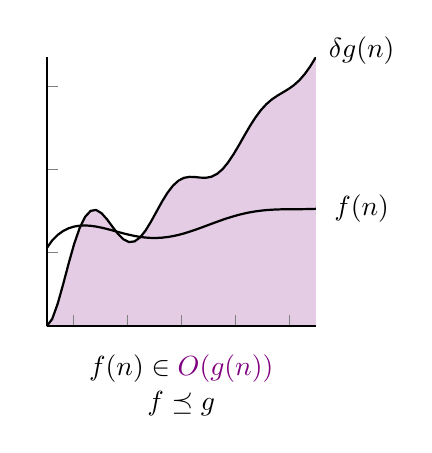
\begin{tikzpicture}
                        \begin{axis}[
                            axis on top=true,
                            axis line style=thick,
                            no markers, domain=1:11, samples=50,
                            axis lines*=left, xlabel=\shortstack{$f(n) \in \violet{O(g(n))}$\\$f \preceq g$}, ylabel=,
                            height=5cm, width=5cm,
                            enlargelimits=false,
                            xticklabels={,,},
                            yticklabels={,,}
                        ]
                            \addplot[fill=violet!20, draw=none] {10 + 0.2*\x^2 + 10*sin(deg(2*(x - 2)))/x} \closedcycle;
                            \addplot[thick] {10 + 0.2*\x^2 + 10*sin(deg(2*(x - 2)))/x};
                            \addplot[thick] {10 + 0.5*\x + 5*sin(deg(x - 1))/x};
                        \end{axis}
                        \node at (4, 3.5) {$\delta g(n)$};
                        \node at (4, 1.5) {$f(n)$};
                    \end{tikzpicture}
                    \hfill
                    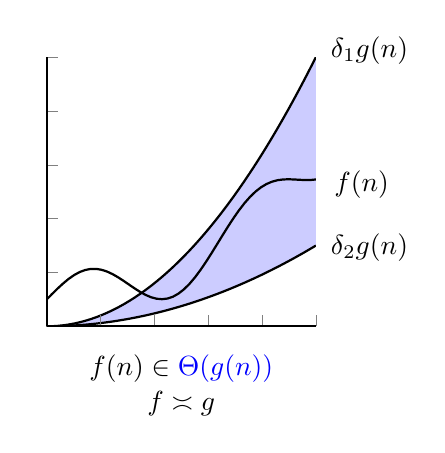
\begin{tikzpicture}
                        \begin{axis}[
                            axis on top=true,
                            axis line style=thick,
                            no markers, domain=0:10, samples=50,
                            axis lines*=left, xlabel=\shortstack{$f(n) \in \blue{\Theta(g(n))}$\\$f \asymp g$}, ylabel=,
                            height=5cm, width=5cm,
                            enlargelimits=false,
                            xticklabels={,,},
                            yticklabels={,,}
                        ]
                            \addplot[fill=blue!20, draw=none] {0.1*\x^2} \closedcycle;
                            \addplot[fill=white, draw=none] {0.03*\x^2} \closedcycle;
                            \addplot[thick] {0.1*\x^2};
                            \addplot[thick] {0.03*\x^2};
                            \addplot[thick] {1 + 0.05*\x^2 + sin(deg(x))};
                        \end{axis}
                        \node at (4.1, 3.5) {$\delta_1 g(n)$};
                        \node at (4.1, 1) {$\delta_2 g(n)$};
                        \node at (4, 1.8) {$f(n)$};
                    \end{tikzpicture}
                    \hfill
                    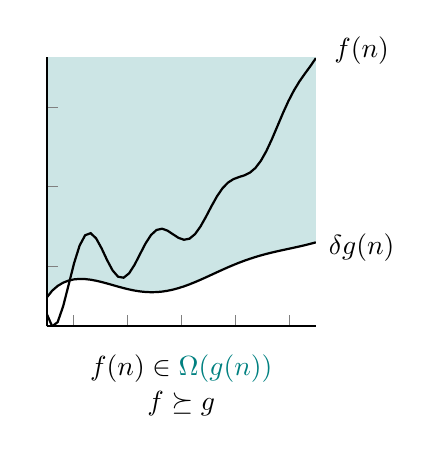
\begin{tikzpicture}
                        \begin{axis}[
                            axis on top=true,
                            axis line style=thick,
                            no markers, domain=1:11, samples=50,
                            axis lines*=left, xlabel=\shortstack{$f(n) \in \teal{\Omega(g(n))}$\\$f \succeq g$}, ylabel=,
                            height=5cm, width=5cm,
                            enlargelimits=false,
                            xticklabels={,,},
                            yticklabels={,,}
                        ]
                            \addplot[fill=teal!20, draw=none] {36.3} \closedcycle;
                            \addplot[fill=white, draw=none] {6 + 0.06*\x^2 + 5*sin(deg(x - 1))/x} \closedcycle;
                            \addplot[thick] {10 + 0.02*\x^3 + 10*sin(deg(2.5*(x - 2)))/x};
                            \addplot[thick] {6 + 0.06*\x^2 + 5*sin(deg(x - 1))/x};
                        \end{axis}
                        \node at (4, 3.5) {$f(n)$};
                        \node at (4, 1) {$\delta g(n)$};
                    \end{tikzpicture}
                \end{center}
                If $f$ and $g$ are L-functions, then either;
                \begin{center}
                    $f \in o(g)$, $f \in \Theta(g)$, or $f \in \Omega(g)$
                \end{center}
                Another method of visualising this is as a Venn diagram, with the upper circle being $O(g(n))$, and the lower circle being $\Omega(g(n))$;
                \begin{center}
                    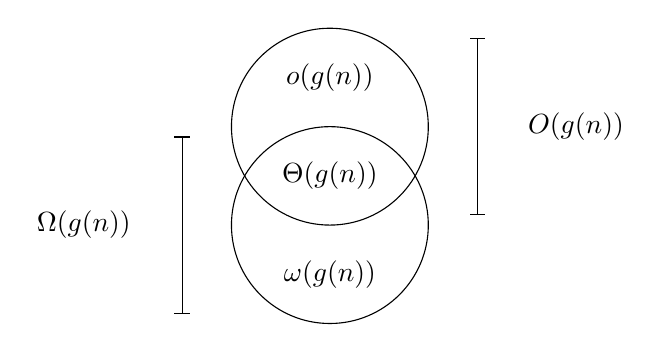
\begin{tikzpicture}[x=1.25cm, y=1.25cm]
                        \draw (0, 0) circle (1);
                        \draw (0, -1) circle (1);
                        \node at (0, 0.5) {$o(g(n))$};
                        \node at (0, -0.5) {$\Theta(g(n))$};
                        \node at (0, -1.5) {$\omega(g(n))$};
                        \node at (2.5, 0) {$O(g(n))$};
                        \node at (-2.5, -1) {$\Omega(g(n))$};
                        \draw
                        (1.5, 0.9) edge[|-|] (1.5, -0.9)
                        (-1.5, -0.1) edge[|-|] (-1.5, -1.9);
                    \end{tikzpicture}
                \end{center}
                Finally, this can also be defined by the following;
                \begin{align*}
                    o(g(n)) & = \{ f \bnfsep \forall \delta > 0.\ \exists n_0 > 0.\ \forall n > n_0.\ |f(n)| < \delta g(n) \} \\
                    O(g(n)) & = \{ f \bnfsep \violet{\exists \delta > 0.\ \exists n_0 > 0.\ \forall n > n_0.\ |f(n)| \leq \delta g(n)} \} \\
                    \Theta(g(n)) & = \left\{f\ \left|\ \begin{matrix}
                        (\violet{\exists \delta > 0.\ \exists n_0 > 0.\ \forall n > n_0.\ |f(n)| \leq \delta g(n)}) \\
                        \land \\
                        (\teal{\exists \delta > 0.\ \forall n_0 > 0.\ \exists n > n_0.\ f(n) \geq \delta g(n)})
                    \end{matrix}\right.\right\} \\
                    & = O(g(n)) \cap \Omega(g(n)) \\
                    \Omega(g(n)) & = \{f \bnfsep \teal{\exists \delta > 0.\ \forall n_0 > 0.\ \exists n > n_0.\ f(n) \geq \delta g(n)}\} \\
                    \omega(g(n)) & = \{ f \bnfsep \forall \delta > 0.\ \forall n_0 > 0.\ \exists n > n_0.\ f(n) > \delta g(n) \}
                \end{align*}
        \subsection*{15th October 2019}
            \subsubsection*{Basic Lists}
                In Haskell, lists are given by \textbf{two} constructors;
                \begin{lstlisting}
                    data [a] = [] | (:) a [a]
                \end{lstlisting}
                This creates two values, called constructors (RHS of data declaration, hence we can pattern match on these unlike other functions);
                \begin{lstlisting}
                    [] :: [a]
                    (:) :: a -> [a] -> [a]
                \end{lstlisting}
                In Haskell, data structures are persistent by default.
                \begin{center}
                    ~[x1,x2,x3] = x1:x2:x3:[]~
                \end{center}
                Visually, we can look at this as "cells" with their constructors and arguments;
                \begin{center}
                    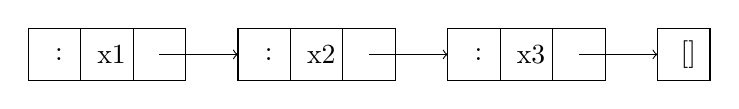
\begin{tikzpicture}[x=0.666cm, y=0.666cm]
                        \begin{scope}[shift={(0, 0)}]
                            \node at (0.5, -0.5) {~:~};
                            \node at (1.5, -0.5) {~x1~};
                            \draw
                            (0, 0) -- (3, 0) -- (3, -1) -- (0, -1) --cycle
                            (1, 0) -- (1, -1)
                            (2, 0) -- (2, -1)
                            (2.5, -0.5) edge[->] (4, -0.5);
                        \end{scope}
                        \begin{scope}[shift={(4, 0)}]
                            \node at (0.5, -0.5) {~:~};
                            \node at (1.5, -0.5) {~x2~};
                            \draw
                            (0, 0) -- (3, 0) -- (3, -1) -- (0, -1) --cycle
                            (1, 0) -- (1, -1)
                            (2, 0) -- (2, -1)
                            (2.5, -0.5) edge[->] (4, -0.5);
                        \end{scope}
                        \begin{scope}[shift={(8, 0)}]
                            \node at (0.5, -0.5) {~:~};
                            \node at (1.5, -0.5) {~x3~};
                            \draw
                            (0, 0) -- (3, 0) -- (3, -1) -- (0, -1) --cycle
                            (1, 0) -- (1, -1)
                            (2, 0) -- (2, -1)
                            (2.5, -0.5) edge[->] (4, -0.5);
                        \end{scope}
                        \node at (12.5, -0.5) {~[]~};
                        \draw (12, 0) -- (13, 0) -- (13, -1) -- (12, -1) --cycle;
                    \end{tikzpicture}
                \end{center}
                Appending lists together is achieved with ~(++)~;
                \begin{lstlisting}
                    (++) :: [a] -> [a] -> [a]
                    [] ++ ys = ys
                    (x:xs) ++ ys = x:(xs ++ ys)
                \end{lstlisting}
                When we do ~xs ++ ys~, the final structure points to ~ys~.
                The trade-off here is that we didn't have to modify ~ys~, but we had to create a new ~x1~, and ~x2~;
                \begin{center}
                    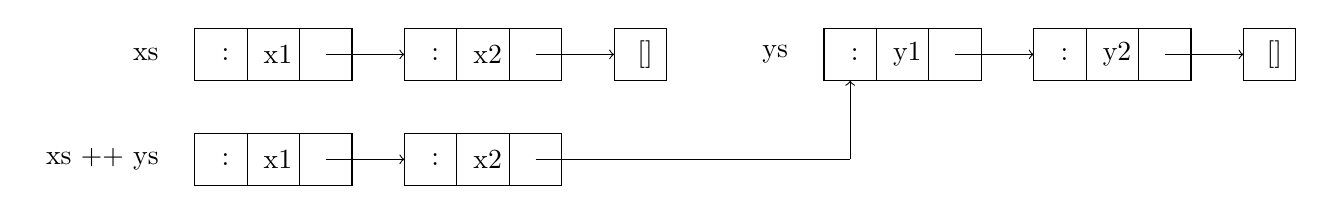
\begin{tikzpicture}[x=0.666cm, y=0.666cm]
                        \begin{scope}[shift={(0, 0)}]
                            \node[anchor=east] at (-0.5, -0.5) {~xs~};
                            \begin{scope}[shift={(0, 0)}]
                                \node at (0.5, -0.5) {~:~};
                                \node at (1.5, -0.5) {~x1~};
                                \draw
                                (0, 0) -- (3, 0) -- (3, -1) -- (0, -1) --cycle
                                (1, 0) -- (1, -1)
                                (2, 0) -- (2, -1)
                                (2.5, -0.5) edge[->] (4, -0.5);
                            \end{scope}
                            \begin{scope}[shift={(4, 0)}]
                                \node at (0.5, -0.5) {~:~};
                                \node at (1.5, -0.5) {~x2~};
                                \draw
                                (0, 0) -- (3, 0) -- (3, -1) -- (0, -1) --cycle
                                (1, 0) -- (1, -1)
                                (2, 0) -- (2, -1)
                                (2.5, -0.5) edge[->] (4, -0.5);
                            \end{scope}
                            \node at (8.5, -0.5) {~[]~};
                            \draw (8, 0) -- (9, 0) -- (9, -1) -- (8, -1) --cycle;
                        \end{scope}
                        \begin{scope}[shift={(12, 0)}]
                            \node[anchor=east] at (-0.5, -0.5) {~ys~};
                            \begin{scope}[shift={(0, 0)}]
                                \node at (0.5, -0.5) {~:~};
                                \node at (1.5, -0.5) {~y1~};
                                \draw
                                (0, 0) -- (3, 0) -- (3, -1) -- (0, -1) --cycle
                                (1, 0) -- (1, -1)
                                (2, 0) -- (2, -1)
                                (2.5, -0.5) edge[->] (4, -0.5);
                            \end{scope}
                            \begin{scope}[shift={(4, 0)}]
                                \node at (0.5, -0.5) {~:~};
                                \node at (1.5, -0.5) {~y2~};
                                \draw
                                (0, 0) -- (3, 0) -- (3, -1) -- (0, -1) --cycle
                                (1, 0) -- (1, -1)
                                (2, 0) -- (2, -1)
                                (2.5, -0.5) edge[->] (4, -0.5);
                            \end{scope}
                            \node at (8.5, -0.5) {~[]~};
                            \draw (8, 0) -- (9, 0) -- (9, -1) -- (8, -1) --cycle;
                        \end{scope}
                        \begin{scope}[shift={(0, -2)}]
                            \node[anchor=east] at (-0.5, -0.5) {~xs ++ ys~};
                            \begin{scope}[shift={(0, 0)}]
                                \node at (0.5, -0.5) {~:~};
                                \node at (1.5, -0.5) {~x1~};
                                \draw
                                (0, 0) -- (3, 0) -- (3, -1) -- (0, -1) --cycle
                                (1, 0) -- (1, -1)
                                (2, 0) -- (2, -1)
                                (2.5, -0.5) edge[->] (4, -0.5);
                            \end{scope}
                            \begin{scope}[shift={(4, 0)}]
                                \node at (0.5, -0.5) {~:~};
                                \node at (1.5, -0.5) {~x2~};
                                \draw
                                (0, 0) -- (3, 0) -- (3, -1) -- (0, -1) --cycle
                                (1, 0) -- (1, -1)
                                (2, 0) -- (2, -1);
                            \end{scope}
                            \draw
                            (6.5, -0.5) -- (12.5, -0.5)
                            (12.5, -0.5) edge[->] (12.5, 1);
                        \end{scope}
                    \end{tikzpicture}
                \end{center}
                Therefore, the complexity is linear, but only depends on ~xs~, and not ~ys~, hence we can say;
                \begin{center}
                    $T_~(++)~ \in O(n)$, where $n = ~length xs~$ in ~xs ++ ys~
                \end{center}
            \subsubsection*{Folding}
                The structure of lists is completed reduced by the ~foldr~ function;
                \begin{lstlisting}
                    foldr :: (a -> b -> b) -> b -> [a] -> b
                    foldr f k [] = k
                    foldr f k (x:xs) = f x (foldr f k xs)
                \end{lstlisting}
                This replaces ~(:)~ with ~f~, and ~[]~ with ~k~;
                \begin{center}
                    \begin{tikzpicture}
                        \begin{scope}[shift={(0, 0)}]
                            \node (o) at (0, 0) {~(:)~};
                            \node (ol) at (-1, -1) {~x1~};
                            \node (or) at (1, -1) {~(:)~};
                            \node (orl) at (0, -2) {~x2~};
                            \node (orr) at (2, -2) {~(:)~};
                            \node (orrl) at (1, -3) {~xn~};
                            \node (orrr) at (3, -3) {~[]~};
                            \draw
                            (o) -- (ol)
                            (o) -- (or)
                            (or) -- (orl)
                            (or) edge[thick, dotted] (orr)
                            (orr) -- (orrl)
                            (orr) -- (orrr);
                        \end{scope}
                        \node at (5, -1.5) {$\overset{~foldr f k~}{\leadsto}$};
                        \begin{scope}[shift={(8, 0)}]
                            \node (o) at (0, 0) {~f~};
                            \node (ol) at (-1, -1) {~x1~};
                            \node (or) at (1, -1) {~f~};
                            \node (orl) at (0, -2) {~x2~};
                            \node (orr) at (2, -2) {~f~};
                            \node (orrl) at (1, -3) {~xn~};
                            \node (orrr) at (3, -3) {~k~};
                            \draw
                            (o) -- (ol)
                            (o) -- (or)
                            (or) -- (orl)
                            (or) edge[thick, dotted] (orr)
                            (orr) -- (orrl)
                            (orr) -- (orrr);
                        \end{scope}
                    \end{tikzpicture}
                \end{center}
                Note that doing ~foldr (:) []~ is the same as ~id~, but with more work, and also ~xs ++ ys~ is equivalent to ~foldr (:) ys xs~.
                Similarly, we have ~foldl~;
                \begin{center}
                    \begin{minipage}[b]{0.55\textwidth}
                        \begin{lstlisting}
                            foldl :: (b -> a -> b) -> b -> [a] -> b
                            foldl f k [] = k
                            foldl f k (x:xs) = foldl f (f k s) xs
                        \end{lstlisting}
                    \end{minipage}
                    \hfill
                    \begin{minipage}[h]{0.4\textwidth}
                        \begin{center}
                            \begin{tikzpicture}[x=-1cm]
                                \node (o) at (0, 0) {~f~};
                                \node (ol) at (-1, -1) {~xn~};
                                \node (or) at (1, -1) {~f~};
                                \node (orl) at (0, -2) {~x2~};
                                \node (orr) at (2, -2) {~f~};
                                \node (orrl) at (1, -3) {~x1~};
                                \node (orrr) at (3, -3) {~k~};
                                \draw
                                (o) -- (ol)
                                (o) edge[thick, dotted] (or)
                                (or) -- (orl)
                                (or) -- (orr)
                                (orr) -- (orrl)
                                (orr) -- (orrr);
                            \end{tikzpicture}
                        \end{center}
                    \end{minipage}
                \end{center}
                Consider a binary operator $(\diamond)$;
                \begin{align*}
                    x \diamond (y \diamond z) & = (x \diamond y) \diamond z & \diamond-\text{associative} \\
                    \epsilon \diamond y & = y & \epsilon-\text{left-unit} \\
                    x \diamond \epsilon & = x & \epsilon-\text{right-unit}
                \end{align*}
                When folding with $\diamond$ and $\epsilon$, ~foldr~ and ~foldl~ coincide.
            \subsubsection*{List Concatenation}
                An application of this is list concatenation, consider ~concat~;
                \begin{lstlisting}
                    concat :: [[a]] -> [a]
                    concat [] = []
                    concat (xs:xss) = xs ++ concat xss
                \end{lstlisting}
                This can be written as a ~foldr~;
                \begin{lstlisting}
                    rconcat :: [[a]] -> [a]
                    rconcat = foldr (++) []
                \end{lstlisting}
                Since ~(++)~ is associate with a neutral element ~[]~, we can write a ~foldl~ version;
                \begin{lstlisting}
                    lconcat :: [[a]] -> [a]
                    lconcat = foldl (++) []
                \end{lstlisting}
                While ~lconcat = rconcat~, this only represents extensional (what values are produced) equality.
                They are not intensionally (how those values are produced) equal.
        \subsection*{18th October 2019}
            \subsubsection*{Concatenation and Associativity}
                The complexity of ~xs ++ ys~ is; $T_~(++)~(m, n) \in O(m)$, where $m = ~length xs~$, and $n = ~length ys~$ - note that it doesn't consider $n$ as expected.
                We want to consider the complexity of;
                $$\overbrace{~(~\underbrace{~(~\overbrace{~(~\underbrace{~(xs~_~1~~++ xs~_~2~~)~}_{n}~ ++ xs~_~3~~)~}^{2n}~ ++ ...)~}_{3n}~ ++ xs~_~m+1~~)~}^{mn}$$
                In lieu of having individual variables, we can approximate all the lists ~xs1~ to $~xs~_~m+1~$ as having the same length $n$.
                This means that if $m = ~length xss~$, then ~concat xss~ has complexity;
                \begin{center}
                    $n + 2n + 3n + \dots + mn = n(1 + 2 + 3 + \dots + m) \in O(nm^2)$
                \end{center}
                If we now look at the right associative version;
                \begin{center}
                    $~xs~_~1~~ ++ (xs~_~2~~ ++ (xs~_~3~~ ++ (... ++ (xs~_~m~~ ++ xs~_~{m+1}~~))))~$
                \end{center}
                Note that each of the ~++~ operations cost $n$, and we have $m$ of them, under the same assumption.
                Therefore, we have $O(mn)$.
                \medskip

                Note that adding to the right of a list is similar to doing the first version, which is left associative, and also more expensive.
                Preferably, we'd add to the left of the list, however this isn't always possible, as we'd also like to be able to add to the right of the list.
            \subsubsection*{Function Composition}
                We do not want to suffer the consequences of poor associativity.
                To solve this, we notice that function composition pays no associativity penalty.
                First note that function composition is as follows;
                \begin{center}
                    ~(f . g) x = f (g x)~
                \end{center}
                We can also show that function composition is both extensionally and intensionally equal, by unrolling the definition;
                \begin{center}
                    ~((f . g) . h) x = f (g (h x))~

                    vs

                    ~(f . (g . h)) x = f (g (h x))~
                \end{center}
                For our lists, we will replace with;
                \begin{center}
                    $~((xs~_~1~~ ++) . (xs~_~2~~ ++) . ... . (xs~_~m+1~~ ++)) []~$
                \end{center}
                Note that each of $~(xs~_~i~~ ++)~$ is a partially applied function that takes a list, and adds $~xs~_~i~$ to the start.
                This is equivalent to the right associative version we had before, which has a better time complexity.
            \subsubsection*{Difference List (DList)}
                The idea is to replace lists with functions that take in a list and give a list back.
                Previously, we'd consider $~xs~_~1~$ a list, but we now use $~(xs~_~1~~ ++)~$, which needs to be applied to the empty list.
                A value of type ~a~ in the list is now a function of type ~[a] -> [a]~.
                We can create a new datatype;
                \begin{lstlisting}
                    data DList a = DList ([a] -> [a])
                \end{lstlisting}
                We need ways of making lists from DLists, and vice versa;
                \begin{lstlisting}
                    -- technically called the abstraction function
                    toList :: DList a -> [a]
                    toList (DList fxs) = fxs []

                    fromList :: [a] -> DList a
                    fromList xs = DList (xs ++)
                    -- or         DList (\ys -> xs ++ ys)
                \end{lstlisting}
                We also need a way of adding DLists together (note the notes use $\diamond$, but I can't really get that with the listing environment, so I will use ~<>~);
                \begin{lstlisting}
                    (<>) :: DList a -> DList a -> DList a
                    DList fxs <> DList fys = DList (fxs . fys)
                    -- or                    DList (\zs -> fxs (fys zs))
                \end{lstlisting}
                Note that taking the head or tail of this list now requires constructing the entire list, which will take linear time.
            \subsubsection*{List Anatomy}
                \begin{center}
                    \begin{tikzpicture}[x=0.1cm]
                        \node[anchor=west] at (0, 0) {$~xs = [x~_~1~~, x~_~2~~, x~_~3~~, ..., x~_~n-1~~, x~_~n~~]~$};
                        \node (h) at (0, 1.25) {~head xs~};
                        \node (c) at (-10, -1) {\shortstack{(~x:~)\\~"cons"~}};
                        \node (l) at (79, -1.25) {~last xs~};
                        \node (s) at (89, 1) {\shortstack{(~++[y]~)\\~"snoc"~}};
                        \draw
                        (h) edge[bend left=20] (16, 0.5)
                        (c) edge[->, bend right=10] (10, -0.2)
                        (l) edge[bend left=20] (63, -0.5)
                        (s) edge[->, bend right=10] (69, 0.2);
                        \draw
                        (14, 0.5) edge[|-|] (18, 0.5)
                        (22, 0.5) edge[|-|, above] node{~tail xs~} (65, 0.5)
                        (65, -0.5) edge[|-|] (61, -0.5)
                        (57, -0.5) edge[|-|, below] node{~init xs~} (14, -0.5);
                    \end{tikzpicture}
                \end{center}
            \subsubsection*{List Interface}
                Rather than dealing with lists directly, we want to work with a specification instead.
                For this, we are creating a type class - an abstraction mechanism that has a class of objects, which have certain operations - and depending on what is given the operations can operate slightly differently.
                \begin{lstlisting}
                    class List list where
                    empty :: list a
                    cons :: a -> list a -> list a
                    snoc :: a -> list a -> list a
                    head :: list a -> a
                    tail :: list a -> list a
                    init :: list a -> list a
                    last :: list a -> a
                    length :: list a -> Int
                    (++) :: list a -> list a -> list a
                    null :: list a -> Bool
                    single :: list a -> Bool

                    toList :: list a -> [a]
                    fromList :: [a] -> list a
                \end{lstlisting}
                Note that ~toList~ and ~fromList~ must behave nicely when composed;
                \begin{center}
                    ~id = toList . fromList~
                \end{center}
                However, composing the functions in reverse does not necessarily yield the same result.
                Consider the case with our DList - it would be perfectly valid to have ~(DList reverse)~; however, since the space of functions is much greater than the space of lists, we cannot reasonably convert ~revert~ into a list, and then hope to get ~reverse~ back out.
                \medskip

                However, we can say that if we had something representing a list, converting it to a list and then back to our implementation of a list, should yield something similar.
                \begin{center}
                    ~normalise = fromList . toList~
                \end{center}
            \subsubsection*{Exercises}
                \begin{enumerate}[1.]
                    \itemsep0em
                    \item Prove formally that $(n + 1)^2 \in \Theta(n^2)$ by exhibiting the necessary constants.
                        \medskip

                        We set $f(n) = (n + 1)^2$, and $g(n) = n^2$.
                        By our definition of $\Theta$, we need to satisfy both the following;
                        \begin{center}
                            $O(g(n)) = \{ f \bnfsep \violet{\exists \delta > 0.\ \exists n_0 > 0.\ \forall n > n_0.\ |f(n)| \leq \delta g(n)} \}$

                            $\Omega(g(n)) = \{f \bnfsep \teal{\exists \delta > 0.\ \forall n_0 > 0.\ \exists n > n_0.\ f(n) \geq \delta g(n)}\}$
                        \end{center}
                        The first case, we want to find $\delta$ such that;
                        \begin{align*}
                            (n + 1)^2 & \leq \delta n^2 & \Leftrightarrow \\
                            n^2 + 2n + 1 & \leq \delta n^2 & \Leftrightarrow \\
                            0 & \leq (\delta - 1) n^2 - 2n - 1 & \text{assuming } \delta - 1 = 3,\ \Rightarrow \\
                            0 & \leq (3n + 1)(n - 1)
                        \end{align*}
                        Hence we have $\delta = 4$.
                        The second case, $\Omega$, is trivial to prove with $\delta = 1$.
                    \item Give examples of expressions that are;
                        \begin{enumerate}[1.]
                            \itemsep0em
                            \item in head normal form, but not in normal form \hfill ~5:take 2 [1,2,3]~
                            \item in weak head normal form, but not in head normal form \hfill ~\ttbs x -> take 2 [1,2,3]~
                            \item in no normal form of any kind \hfill ~take 2 [1,2,3]~
                                \subitem it's not a constructor, and there isn't a $\lambda$-abstraction
                            \item in normal form, but not in weak head normal form \hfill not possible
                        \end{enumerate}
                    \item Using the definition of $f \in O(g(n))$ as a set, derive the definition of $f \in \omega(g(n))$ as a set.
                        \medskip

                        Recall that $f \in \omega(g(n)) \Leftrightarrow f \notin O(g(n))$, and the following definition;
                        \begin{center}
                            $O(g(n)) = \{ f \bnfsep \exists \delta > 0.\ \exists n_0 > 0.\ \forall n > n_0.\ |f(n)| \leq \delta g(n) \}$
                        \end{center}
                        Using equivalences for first-order logic;
                        \begin{align*}
                            & \neg \exists \delta > 0.\ \exists n_0 > 0.\ \forall n > n_0.\ |f(n)| \leq \delta g(n) \\
                            \equiv\ & \forall \delta > 0.\ \neg \exists n_0 > 0.\ \forall n > n_0.\ |f(n)| \leq \delta g(n) \\
                            \equiv\ & \forall \delta > 0.\ \forall n_0 > 0.\ \neg \forall n > n_0.\ |f(n)| \leq \delta g(n) \\
                            \equiv\ & \forall \delta > 0.\ \forall n_0 > 0.\ \exists n > n_0.\ \neg(|f(n)| \leq \delta g(n)) \\
                            \equiv\ & \forall \delta > 0.\ \forall n_0 > 0.\ \exists n > n_0.\ f(n) > \delta g(n)
                        \end{align*}
                        Hence we can write $\omega$ as the following;
                        \begin{center}
                            $\omega(g(n)) = \{ f \bnfsep \forall \delta > 0.\ \forall n_0 > 0.\ \exists n > n_0.\ f(n) > \delta g(n) \}$
                        \end{center}
                    \item
                        The composition rule gives the time complexity of two functions $f$ and $g$ when they are composed.
                        By using the definition of $e^T$, derive the accurate cost of $f\ (g\ x)$ using strict evaluation.
                        \begin{align*}
                            ((f \circ g)\ x)^T & = 1 + (f(g(x)))^T \\
                            & = 1 + f^T(g(x)) + (g(x))^T \\
                            & = 1 + f^T(g(x)) + g^Tx + x^T \\
                            & = 1 + f^T(g(x)) + g^Tx
                        \end{align*}
                    \item Justify whether each of the following is true or false;
                        \begin{enumerate}[1.]
                            \itemsep0em
                            \item $2n^2 + 3n \in \Theta(n^2)$ \hfill true
                            \item $2n^2 + 3n \in O(n^3)$ \hfill true
                            \item $n\log n \in O(n\sqrt{n})$ \hfill ($\log n$ grows slower than $\sqrt{n}$) true
                            \item $n + \sqrt{n} \in O(n\log n)$ \hfill false
                            \item $2^{\log n} \in O(n)$ \hfill (use laws of logarithms) true
                        \end{enumerate}
                \end{enumerate}
\end{document}